\documentclass[sigconf]{acmart}

\usepackage{booktabs}
\usepackage{multirow}
\usepackage{graphicx}
\usepackage{microtype}
\usepackage{algorithm}
\usepackage{algpseudocode}

\AtBeginDocument{%
  \providecommand\BibTeX{{%
    Bib\TeX}}}

\acmConference[ECS 172]{Recommender Systems}{Spring 2026}{University of California, Davis}

% Course project, not an ACM publication: suppress the copyright/permission
% block, placeholder ISBN/DOI, and the auto-generated ACM reference box.
\setcopyright{none}
\settopmatter{printacmref=false}
% Empty the first-page copyright footnote entirely (removes the leftover
% venue line, "ACM ISBN ...", and "https://doi.org/..." placeholders).
\renewcommand\footnotetextcopyrightpermission[1]{}

\begin{document}

\title{Can Recommending Real-World Interrogation Techniques Help LLMs Moderate Extremist Views?}

\author{Bill Steeven Koumba Moussadji Lu}
\affiliation{\institution{University of California, Davis}\city{Davis}\state{CA}\country{USA}}
\email{bkoumbamoussadjilu@ucdavis.edu}

\author{Sanjay Manivasagam}
\affiliation{\institution{University of California, Davis}\city{Davis}\state{CA}\country{USA}}
\email{sanmanivas@ucdavis.edu}

\author{Marcin Wróblewski}
\affiliation{\institution{University of California, Davis}\city{Davis}\state{CA}\country{USA}}
\email{mawroblewski@ucdavis.edu}

\author{Haoyu Yan}
\affiliation{\institution{University of California, Davis}\city{Davis}\state{CA}\country{USA}}
\email{yhyyan@ucdavis.edu}

% ─────────────────────────────────────────────────────────────────────────────
\begin{abstract}
Moderating extremist or entrenched views online remains a persistent challenge.
We ask whether a retrieval-augmented generation (RAG) recommender that selects
real-world interrogation and debate techniques at each conversational turn can
produce more reliably \emph{directed} stance change in a simulated LLM suspect
than an unguided baseline. We build a three-role system (Suspect, Interrogator, and
Judge) and evaluate it with a quad experimental design (matched control and
treatment pairs) across four ballot-measure topics, including one drawn from
verbatim arguments of the Davis Measure V June 2026 special election. Across 80
experimental legs, the treatment interrogator achieves \textbf{75\% directional
accuracy} versus \textbf{35\%} for the unguided control, a 40-percentage-point
improvement ($p<0.001$). Pooled stance-change \emph{magnitude}, by contrast, is
nearly identical across conditions: the effect is on the direction and
smoothness of movement, not its size. The largest single-topic gap is Transit (10\%
$\to$ 90\%). Measure V, our real-data condition, replicates the gain (30\%
$\to$ 70\%), confirming that technique recommendation transfers to genuine
public-debate arguments. These results suggest that RAG-guided technique
recommendation is a viable component for LLM-based persuasion and moderation
systems.
\end{abstract}

\keywords{retrieval-augmented generation, recommender systems, stance change,
LLM agents, content moderation, persuasion}

\maketitle

% ─────────────────────────────────────────────────────────────────────────────
\section{Introduction}

The proliferation of online extremism and entrenched misinformation has
motivated sustained research into automated moderation~\cite{kumar2023language,
gorwa2020algorithmic}. Most deployed systems operate at the content level
(flagging, removing, or down-ranking objectionable posts) but do not attempt to
change the underlying beliefs that motivate harmful speech. A growing body of
work instead explores \emph{conversational intervention}: engaging an individual
in dialogue to shift their stated position~\cite{costello2024durably}. Early
results are promising but rely on general-purpose language models with no
principled mechanism for selecting which argumentative strategy to deploy next.
This work is situated within a broader research vision of AI as a facilitator of
constructive dialogue and healthy discourse, one that addresses polarized views
not by removing speech after the fact, but by engaging with the underlying beliefs
that motivate it.

Recommender systems offer a natural framing for this problem. The
\emph{query} is the suspect's current conversational state (most recent
utterance, inferred values, running argument history); the \emph{item catalog}
is a curated corpus of interrogation and debate techniques drawn from
professional practice; and the \emph{recommendation} drives the interrogator's
next move. This framing connects to the broader RAG literature, where retrieved
context improves generation quality~\cite{izacard2022few}, and to multi-agent
debate research, where structured disagreement improves LLM
reasoning~\cite{estornell2024scaling}.

\medskip
We make the following contributions:
\begin{itemize}
  \item A three-role multi-agent architecture (Suspect, Interrogator, Judge)
    with a two-channel RAG recommender: one channel for technique selection
    and one for topic-aligned argument retrieval.
  \item A \emph{quad experimental design} that pairs direction-matched control
    and treatment legs, enabling within-quad comparison that mitigates judge
    scaling bias.
  \item An evaluation across four ballot-measure topics including one using
    verbatim real-world arguments (Davis Measure V, June 2026), demonstrating
    that technique recommendation generalizes beyond synthetic data.
  \item Empirical evidence that the two-channel RAG recommender (technique
    \emph{and} argument retrieval together) improves directional accuracy from
    35\% to 75\% across 80 experimental legs ($p<0.001$, pooled). We are explicit
    that the design does not isolate the technique channel from the argument
    channel; an arguments-only ablation is the most important follow-up experiment.
\end{itemize}

% ─────────────────────────────────────────────────────────────────────────────
\section{Related Work}

\subsection{Conversational Persuasion and Stance Change}
Costello et al.~\cite{costello2024durably} show that a single AI-driven
conversation can durably reduce conspiracy beliefs, with effects persisting
two months later. Their approach uses a general-purpose LLM without a curated
technique corpus. Our work extends this by asking whether a \emph{recommender}
that selects among professionally documented techniques can improve on the
unguided baseline. Where Costello et al.\ treat persuasion strategy as implicit
in the model's pretraining, we make strategy selection an explicit recommendation
problem, separating the choice of technique from its execution so that each can
be controlled and studied independently.

\subsection{LLM-Based Content Moderation}
Kumar et al.~\cite{kumar2023language} demonstrate that instruction-tuned LLMs
outperform traditional classifiers on toxicity detection but remain sensitive
to context shifts. Hong et al.~\cite{hong2024curiosity} show through
curiosity-driven red-teaming that LLMs can be induced to produce unsafe outputs
under adversarial prompts, motivating the need for robust intervention
mechanisms beyond passive filtering. Our work complements this detection-oriented
line by operating at a different layer: rather than flagging content after it
appears, we attempt to shift the underlying beliefs that produce it, a proactive
complement to reactive content moderation. Adaptively recommending techniques at
each turn may also contribute a form of robustness: a structured technique corpus
constrains the interrogator's behaviour, reducing the risk of an LLM spiralling
into incoherent or off-target responses when the conversation takes an unexpected
turn.

\subsection{Multi-Agent Debate}
Estornell and Liu~\cite{estornell2024scaling} study multi-agent debate as a
mechanism for improving LLM reasoning quality. They find that when participating
models share similar capabilities or come from the same training distribution,
debates can stall: rather than reaching better answers through disagreement,
agents converge on the majority opinion embedded in their shared training
data, including shared misconceptions. This means that adding more debating
agents does not guarantee correctness when all agents share the same blind spots.
Unlike Estornell and Liu's multi-agent reasoning setup, our system uses
structured dialogue for belief intervention rather than answer verification.
However, our use of a single model family (llama3.1:8b) for all three roles
introduces the same shared-bias concern; we treat this as a known limitation.

\subsection{Retrieval-Augmented Generation}
Izacard et al.~\cite{izacard2022few} establish that retrieved passages
substantially improve generation on knowledge-intensive tasks; this grounding
motivates both retrieval channels in our system. We extend standard RAG in one
respect: retrieval is \emph{turn-aware}. Rather than querying a fixed index,
our phase-filtered technique recommender (Section~\ref{sec:phase}) changes which
techniques are eligible as the conversation advances, a constraint we draw from
interrogation practice rather than from the retrieval literature.

\subsection{Network Science and Influence Propagation}
Ribeiro et al.~\cite{ribeiro2018sheep} characterize hateful user communities on
Twitter and find that such users are not isolated actors: they form tightly
connected communities with high centrality in retweet networks, with a small
number of high-centrality accounts responsible for a disproportionate share of
content propagation. Yu et al.~\cite{yu2023dygformer} and Sun et
al.~\cite{sun2023explicit} provide dynamic graph-learning tools that model how
influence propagates through such networks over time. Together, these findings
suggest a natural upstream component for systems like ours: using network
analysis to identify high-centrality individuals before initiating dialogue,
rather than waiting for organic encounter. Our current evaluation does not
include this targeting stage; we return to it in the Future Work discussion.

% ─────────────────────────────────────────────────────────────────────────────
\section{System Design}

\subsection{Three-Role Architecture}
The system comprises three LLM roles, each running as a stateful agent against
a local Ollama instance (llama3.1:8b throughout, 180 s per call timeout):

\textbf{Suspect.} Initialized at one of the two stance \emph{poles}, chosen at
random ($d_0 \in \{-2, +2\}$: strongly against or strongly for), together with a
latent persona (values, communication style, and position on the topic), and a
bank of aligned arguments drawn from the topic card (a structured YAML file
that encodes the debate question, arguments for both sides, and suspect values;
see Section~\ref{sec:rag}). The Suspect responds in character and updates its internal model as the
dialogue progresses. Only arguments consistent with the current stance are
surfaced (\texttt{aligned\_only} mode), preventing incoherent position reversals
mid-utterance.

\medskip
\textbf{Interrogator.} Operates in one of two conditions:
\begin{itemize}
  \item \emph{Control:} Receives only the topic question and Suspect utterance;
    no technique guidance.
  \item \emph{Treatment:} Runs a two-stage RAG pipeline
    (Section~\ref{sec:treatment}) that retrieves a technique recommendation and a
    topic-aligned counter-argument before generating each response.
\end{itemize}
Because the control receives \emph{neither} retrieval channel, this contrast
measures the \emph{combined} effect of technique guidance and grounded argument
retrieval. It does not, on its own, isolate the contribution of technique
selection from that of argument retrieval. We are explicit about this
throughout and identify the missing arguments-only condition as the most
important follow-up experiment (Section~\ref{sec:limits}).

\textbf{Judge.} Scores each Suspect utterance on a five-point scale from
$-2$ (strong disagreement) to $+2$ (strong agreement) against the topic
proposition. Scoring is batched across all legs of a quad in a single call to
ensure a consistent scale; out-of-range outputs are clamped and a per-utterance
fallback is used when batch decoding fails (see Section~\ref{sec:robustness}).

\subsection{Technique Corpus}

The technique corpus consists of 18 Markdown cards drawn from three
professional frameworks: the Reid Technique (5 cards covering confrontation,
minimization, and theme development), the Scharff Elicitation Technique
(7 cards), and structured academic debate (6 cards covering steelmanning,
objection handling, and Socratic questioning). Each card is structured with
YAML front-matter followed by a prose body. An example front-matter is shown
below:

\begin{verbatim}
---
name: Rapport Building
phase: early
triggers:
  - beginning of a conversation before position
    has been established
  - suspect appears suspicious of motives
pairs_with: [orbit, oars, motivational_interviewing]
in_tension_with: [surfacing_contradictions,
                  scharff_technique]
out_of_bounds:
  - Do not manufacture false common ground
  - Do not skip rapport-building in favour of
    immediate persuasion — it consistently backfires
---
\end{verbatim}

The \texttt{phase} field constrains when a card is eligible for retrieval;
\texttt{pairs\_with} and \texttt{in\_tension\_with} encode compatibility
metadata that the Stage-1 selector uses to choose a complementary technique;
\texttt{out\_of\_bounds} constraints are passed verbatim to the Stage-2
generator as hard guardrails.

\subsection{Two-Channel RAG Recommender}
\label{sec:rag}

\textbf{Infrastructure.} All 18 technique card bodies and all topic arguments
are stored in ChromaDB, a persistent vector database that supports approximate
nearest-neighbor search over dense embeddings. At each conversational turn,
ChromaDB returns the $k$ most semantically similar documents to the current
query; retrieval latency is negligible relative to the cost of LLM generation.

Documents are embedded with \texttt{all-MiniLM-L6-v2}, a sentence-transformer
model chosen for two practical reasons: (1) it runs entirely on CPU with no
network dependency, matching our offline Ollama setup, and (2) its 384-dimensional
embeddings are well-suited to short, precise prose, matching the format of
both technique card bodies (50--400 tokens) and individual debate arguments. A
domain-adapted embedding model trained on interrogation or debate corpora would
likely improve retrieval precision, particularly for nuanced state distinctions
such as ``suspect is deflecting'' versus ``suspect is emotionally engaged''; we
treat this as a direction for future work.

\textbf{Channel 1: Technique Recommender.} The bodies of the 18 technique cards
are embedded individually and stored in a dedicated collection. At each turn, the
query is the concatenation of the Suspect's latest utterance with the most recent
conversation context. After phase
filtering (Section~\ref{sec:phase}), the top-$k{=}5$ semantically matching
technique cards are retrieved. The value $k{=}5$ was chosen to give the
Stage-1 selector meaningful choice across the available phase-eligible cards
(typically 6--10 after filtering) without diluting the relevance signal. Passing
fewer candidates ($k{=}2$) risks missing a well-matched technique; more
($k{=}8$) risks including cards whose trigger conditions do not match the
current conversational state.

\textbf{Channel 2: Argument Recommender.} Each topic card contributes
argument strings for both sides, embedded individually. The top-$k{=}3$
arguments aligned with the Interrogator's stance are retrieved per turn.
$k{=}3$ keeps the Stage-2 generator focused: more arguments risk introducing
conflicting rhetorical frames, while fewer risk missing the most contextually
relevant counter-argument. Both $k$ values were selected heuristically given
our corpus scale and were not swept; sensitivity analysis is left for future
work.

\subsection{Treatment Pipeline: Two-Stage Recommendation}
\label{sec:treatment}

The treatment Interrogator separates \emph{strategy selection} from
\emph{response generation} into two sequential LLM calls. This separation is a
deliberate design choice: selection requires analytical reasoning (classify the
suspect's orientation, rank techniques, decide persona disclosure), while
generation requires fluent, naturalistic output. Combining both into one call
risks the generator drifting from the selected technique under the pressure of
producing fluent text. The two-stage structure also makes the system modular:
swapping the topic card changes the argument bank without affecting the selector
logic, and the selector can be retargeted to a new technique corpus without
touching the generator prompt.

Algorithms~\ref{alg:control} and~\ref{alg:treatment} contrast the two
conditions:

\begin{algorithm}
\caption{Control Interrogator (per turn)}
\label{alg:control}
\begin{algorithmic}[1]
\Require topic question $Q$, conversation history $H$, suspect utterance $u$
\Ensure interrogator response $r$
\State Append $u$ to $H$
\State $r \leftarrow \mathrm{LLM}(\text{sys}=\text{ControlPrompt}(Q),\; H)$ \Comment{sys: system prompt built from $Q$}
\State Append $r$ to $H$
\State \Return $r$
\end{algorithmic}
\end{algorithm}

\begin{algorithm}
\caption{Treatment Interrogator (per turn)}
\label{alg:treatment}
\begin{algorithmic}[1]
\Require topic card $C$, history $H$, suspect utterance $u$, turn $t$, budget $T$,
         suspect model $\mathcal{M}$, persona state $\mathcal{P}$
\Ensure interrogator response $r$
\State $\text{phase} \leftarrow \mathrm{PhaseOf}(t, T)$
  \Comment{opening / middle / closing}
\State $\mathbf{T}_{\text{top}} \leftarrow \mathrm{ChromaDB.query}(u \oplus H,\; k{=}5,\; \text{filter=phase})$
  \Comment{Channel 1; $u \oplus H$: suspect utterance concatenated with recent history}
\State $\mathbf{A}_{\text{top}} \leftarrow \mathrm{ChromaDB.query}(u,\; k{=}3,\; \text{side=int\_stance})$
  \Comment{Channel 2}
\State Append $u$ to $H$
\State \textbf{Stage 1 (Selector):}
\State $S \leftarrow \mathrm{LLM}(\text{SelectorPrompt},\; H,\; \mathcal{M},\; \mathcal{P},\; \mathbf{T}_{\text{top}},\; \mathbf{A}_{\text{top}})$
  \Comment{JSON: technique, orientation, persona reveal}
\State Update $\mathcal{M}$ with orientation, inferred values, new arguments from $S$
\State Update $\mathcal{P}$: move disclosed detail from latent to revealed
\State \textbf{Stage 2 (Generator):}
\State $r \leftarrow \mathrm{LLM}(\text{GeneratorPrompt},\; H,\; S.\text{technique},\; \mathbf{A}_{\text{top}},\; \mathcal{P}.\text{revealed})$
\State Append $r$ to $H$
\State \Return $r$
\end{algorithmic}
\end{algorithm}

\textbf{Two-channel combination in Stage 2.} Both channels' outputs are passed
simultaneously to the Stage-2 generator: the full prose body and out-of-bounds
constraints of the selected technique card (Channel~1), and the top-3 argument
strings as an ``available to deploy'' list (Channel~2). The generator has
discretion over argument usage: it may rephrase a retrieved argument
positively, ignore it if it would create tension with the selected technique,
or surface it indirectly using the \emph{Scharff framing} described below. For
example, if Channel~1 selects \emph{Rapport Building} (which discourages direct
challenge) and Channel~2 retrieves a sharp factual rebuttal, the generator
typically softens the rebuttal into a curiosity-driven observation.

\textbf{Scharff-style indirect argument deployment.} The Stage-2 generator is
instructed to deploy retrieved arguments indirectly rather than citing them
as facts. This reflects the Scharff Technique, developed by WWII German
intelligence officer Hanns Scharff and later formalized by Oleszkiewicz,
Granhag, and Kleinman~\cite{oleszkiewicz2014scharff}: instead of asking
direct questions (which reveal what the interrogator does not know) or stating
facts (which trigger counter-argument), the interrogator implies familiarity
and invites the suspect to fill in gaps. In our setting this means framing
retrieved arguments as things the Interrogator has ``noticed'' or ``heard
others say'' (\textit{``I've seen that the affordability numbers on similar
projects tend to shift once you factor in the subsidized units\ldots''}),
rather than as direct rebuttals. This keeps the conversation feeling like
collaborative exploration rather than persuasion, which reduces the Suspect's
defensive responses.

\subsection{Phase-Filtered Retrieval}
\label{sec:phase}

Technique retrieval is phase-aware: the current turn number is mapped to a
conversational phase (\texttt{opening}: turns 1--2, \texttt{middle}: 3--4,
\texttt{closing}: 5--6), and technique cards whose \texttt{phase} annotation
does not match are excluded before the semantic search. This design reflects
established practice in professional interrogation: rapport-building is most
effective before substantive disagreement is introduced; challenge techniques
(e.g., Surfacing Contradictions, Cognitive Dissonance) require trust to have
been established and are counterproductive in opening turns; closing techniques
focus on consolidation rather than new information. Enforcing phase-appropriate
retrieval also keeps evaluations to a practical 6-turn length, consistent with
real online conversations, which rarely sustain a single debate thread much
longer. We do not report a controlled comparison between phased and unphased retrieval
(i.e., an experiment that disables the phase filter while holding all else constant);
this is acknowledged as a limitation.

\subsection{Robustness Fixes}
\label{sec:robustness}
During evaluation on the Measure V topic, whose proposition is substantially
longer than the synthetic topics, the Judge LLM occasionally produced
out-of-range scores (e.g., 8 on a $[-2, 2]$ scale) or returned arrays of
incorrect length. We address this with two fixes: (1) numeric scores outside
$[-2, 2]$ are clamped to the nearest valid value, preserving ordinal intent;
(2) if batch scoring fails after three retries, a per-utterance fallback scores
each statement individually. Each quad is scored in two direction-matched
batches (the quad structure is defined in Section~\ref{sec:quad}), so a topic of
5 quads incurs 10 scoring calls; the fallback triggered
on 2 of the 10 calls for Measure V, and those results are included without
special treatment.

% ─────────────────────────────────────────────────────────────────────────────
\section{Experimental Design}

\subsection{Quad Structure}
\label{sec:quad}
Each experimental unit is a \emph{quad}: four legs run from the same seed,
varying condition (control / treatment) and initial suspect direction ($-2$ or
$+2$). Direction-matching across conditions ensures that observed differences
are attributable to the treatment rather than to stance-initial effects.
Legs within a quad are scored in matched pairs (legs 0 \& 2, legs 1 \& 3)
by the same Judge call, enforcing a consistent scoring scale within each
direction.

\subsection{Topics and Dataset}
We evaluate on four topics derived from real ballot measures:

\begin{itemize}
  \item \textbf{Housing (Rezoning)}: composite based on California rezoning
    ballot measures.
  \item \textbf{Arts (Funding)}: composite based on municipal arts levy
    ballot measures.
  \item \textbf{Transit (Fare-free)}: composite based on fare-free transit
    ballot measures including Kansas City (2020).
  \item \textbf{Measure V (Village Farms, Davis)}: verbatim arguments from
    the Yolo County ACE Department for the City of Davis June 2, 2026 Special
    Municipal Election. This is our real-data condition.
\end{itemize}

The first three topics use synthesized argument banks modeled after real
measures; Measure V uses verbatim supporter and opponent arguments as published
by the election authority. All four topics share the same YAML schema
and are processed identically by the pipeline.

\subsection{Metrics}
The Judge scores every suspect utterance, not just the final one. In a
6-turn conversation this yields a trajectory of 7 scores:
$s_0, s_1, \ldots, s_6$, where $s_0$ is the Judge's score of the opening
utterance (before the Interrogator has spoken) and $s_1$--$s_6$ follow each
subsequent suspect reply. Note that $s_0$ is \emph{measured}, not assigned: it
is the Judge's reading of what the suspect actually says first, which need not
equal the assigned pole $d_0$. We compute three metrics over this trajectory:

\textbf{Magnitude.} $|s_6 - s_0|$. The absolute net shift from the
suspect's opening stance to their final stance, regardless of direction.
The scale runs from 0 to 4; a magnitude of 2.10 means the suspect moved
roughly two full points on average.

\textbf{Directional Accuracy.} Fraction of legs where
$\text{sign}(s_6 - s_0)$ matches the Interrogator's target direction, i.e.,
the suspect moved \emph{toward} the Interrogator's position. At 0\% the suspect
never moved toward the Interrogator (it held its ground or moved away); at 100\%
it always did; 50\% corresponds to direction-agnostic drift. Because our claim is
comparative (treatment against its matched control, rather than against an
absolute threshold), this metric is robust to the Judge's scale drift: it depends
only on the sign of each shift, not its magnitude. This is our primary metric.

\textbf{Consistency.} Variance of $s_0, s_1, \ldots, s_6$ within a single
trial. Lower variance means the suspect's stance evolved smoothly or held
steady; higher variance indicates erratic flip-flopping between turns.
Two trials can share the same final magnitude and direction yet differ
sharply in consistency: a trajectory of $[-1, -1, -2]$ (smooth, low
variance) is qualitatively different from $[-1, +1, -1]$ (oscillating,
high variance) even if both end at $-1$. Per-turn scoring makes this
distinction measurable.

\subsection{Scale}
We run 5 quads per topic $\times$ 4 legs per quad $\times$ 6 turns per leg
$= 120$ dialogue turns per topic, 480 turns total. Each topic produces 20 legs
(10 control, 10 treatment). The pooled analysis uses all 80 legs (40 per
condition).

\textbf{Reproducibility.} All four model calls per turn (suspect, interrogator
selector, interrogator generator, judge) use \texttt{llama3.1:8b} through a local
Ollama server at its default decoding settings (temperature 0.8), with a fixed
integer seed supplied on every call. The five quads of a topic use seeds
42--46; within a quad all four legs share the quad's seed, and the same five
seeds recur across the four topics. Given the seed, runs are deterministic.

% ─────────────────────────────────────────────────────────────────────────────
\section{Results}

\subsection{Per-Topic Results}

Table~\ref{tab:results} reports per-topic metrics. Figure~\ref{fig:fig3}
visualizes directional accuracy by condition and topic.

\begin{table}[h]
\centering
\caption{Per-topic metrics by condition. Dir.\,Acc. = directional accuracy
(\% of legs in which the suspect moved toward the Interrogator). Cons. =
consistency (within-trial stance variance; lower = smoother trajectory).}
\label{tab:results}
\begin{tabular}{llrrr}
\toprule
Topic & Condition & Mag. & Dir.\,Acc. & Cons. \\
\midrule
\multirow{2}{*}{Housing}
  & Control   & 2.30 & 40\% & 1.83 \\
  & Treatment & 1.60 & \textbf{80\%} & 1.09 \\
\midrule
\multirow{2}{*}{Arts}
  & Control   & 1.50 & 60\% & 1.30 \\
  & Treatment & 1.80 & 60\% & 1.08 \\
\midrule
\multirow{2}{*}{Transit}
  & Control   & 1.20 & 10\% & 1.30 \\
  & Treatment & 2.10 & \textbf{90\%} & 1.27 \\
\midrule
\multirow{2}{*}{Measure V}
  & Control   & 2.00 & 30\% & 1.65 \\
  & Treatment & 1.60 & \textbf{70\%} & 1.16 \\
\midrule
\multirow{2}{*}{\textbf{Pooled}}
  & Control   & 1.75 & 35\% & 1.52 \\
  & Treatment & 1.77 & \textbf{75\%} & 1.15 \\
\bottomrule
\end{tabular}
\end{table}

\textbf{Directional accuracy.} The headline result is the \emph{pooled} gap:
treatment legs move toward the Interrogator in 30 of 40 cases (75\%) versus 14 of
40 (35\%) for control. A two-proportion test on these counts gives $z=3.6$,
$p<0.001$, so the gap is very unlikely to be sampling noise. We lead with the
pooled comparison deliberately: per-topic differences rest on only $n=10$ legs
per condition, whose 95\% confidence intervals span roughly $\pm30$ percentage
points, and we therefore treat individual topic rankings as indicative rather
than reliable. With that caveat, treatment exceeds control on 3 of 4 topics
(Housing, Transit, Measure V) and ties on Arts (60\% vs.\ 60\%). The pooled test
does carry one qualification: the five seeds recur across topics and the two
conditions are matched within a quad, so the legs are not fully independent; a
larger fully-crossed run would tighten this estimate.

\textbf{Transit} shows the largest nominal gap (control 10\%, treatment 90\%),
but at $n=10$ this single-topic number is the least certain in the paper and we
do not build any claim on it alone. It does, however, surface a pattern visible
across topics: control accuracy is frequently \emph{below} 50\%. We examine that
in Section~\ref{sec:control}.

\textbf{Measure V} (real data) mirrors the Housing result exactly: $+40$pp
directional accuracy improvement. Despite having a much longer, more complex
proposition and 17+ arguments per side (vs.\ 5 in the synthetic topics), the
treatment pipeline produces the same magnitude of improvement. This confirms
that the technique recommender generalizes to real-world argument corpora.

\textbf{Arts} is the only topic where treatment does not improve over control.
We attribute this to the nature of arts-funding arguments, which tend toward
values-based appeals (equity, culture, community) rather than factual claims.
The techniques retrieved here lean toward the Reid and Scharff frameworks, which
target factual-claim disputes; why the corpus's values-applicable debate cards
did not close the gap is examined in the Discussion.

\subsection{Magnitude and Consistency}

Magnitude effects are mixed (Figure~\ref{fig:fig1}): Transit shows a strong
positive effect (+0.90), while Housing ($-0.70$) and Measure V ($-0.40$) show
negative effects. We
caution against over-interpreting magnitude results: the Judge LLM
(llama3.1:8b) exhibits scale drift on complex or politically charged
propositions, assigning systematically higher or lower absolute scores
regardless of the actual stance. Directional accuracy, which depends only on
the sign of the final shift, is substantially less sensitive to this artifact
and is therefore our primary metric.

Consistency (within-trial stance variance) is uniformly lower in treatment
legs ($\approx 1.15$) than control ($\approx 1.52$). Lower variance means
the suspect's stance shifted smoothly rather than flip-flopping between
turns, consistent with genuine directional influence. The control
interrogator, lacking technique guidance, appears to provoke resistance on
some turns and concession on others, producing oscillation; the
RAG-guided interrogator produces more monotonic trajectories
(Figure~\ref{fig:fig2}).

\subsection{Figures}

\begin{figure}[h]
  \centering
  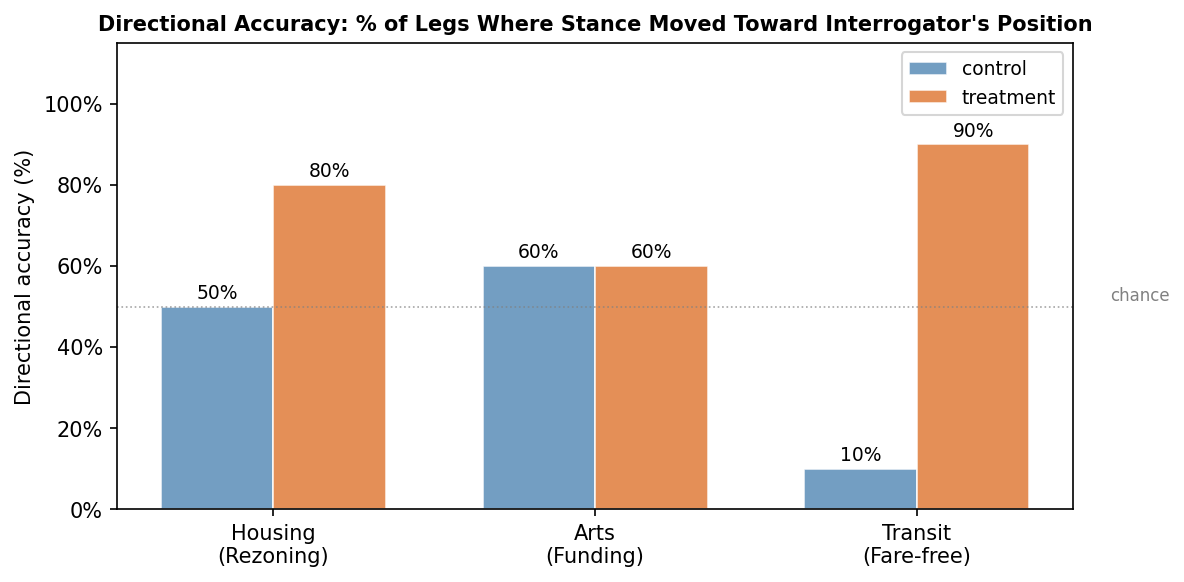
\includegraphics[width=\linewidth]{../results/figures/fig3_directional_accuracy.png}
  \caption{Directional accuracy (\%) by topic and condition. The dashed line at
    50\% marks direction-agnostic drift. Treatment exceeds control on 3 of 4 topics.}
  \label{fig:fig3}
\end{figure}

\begin{figure}[h]
  \centering
  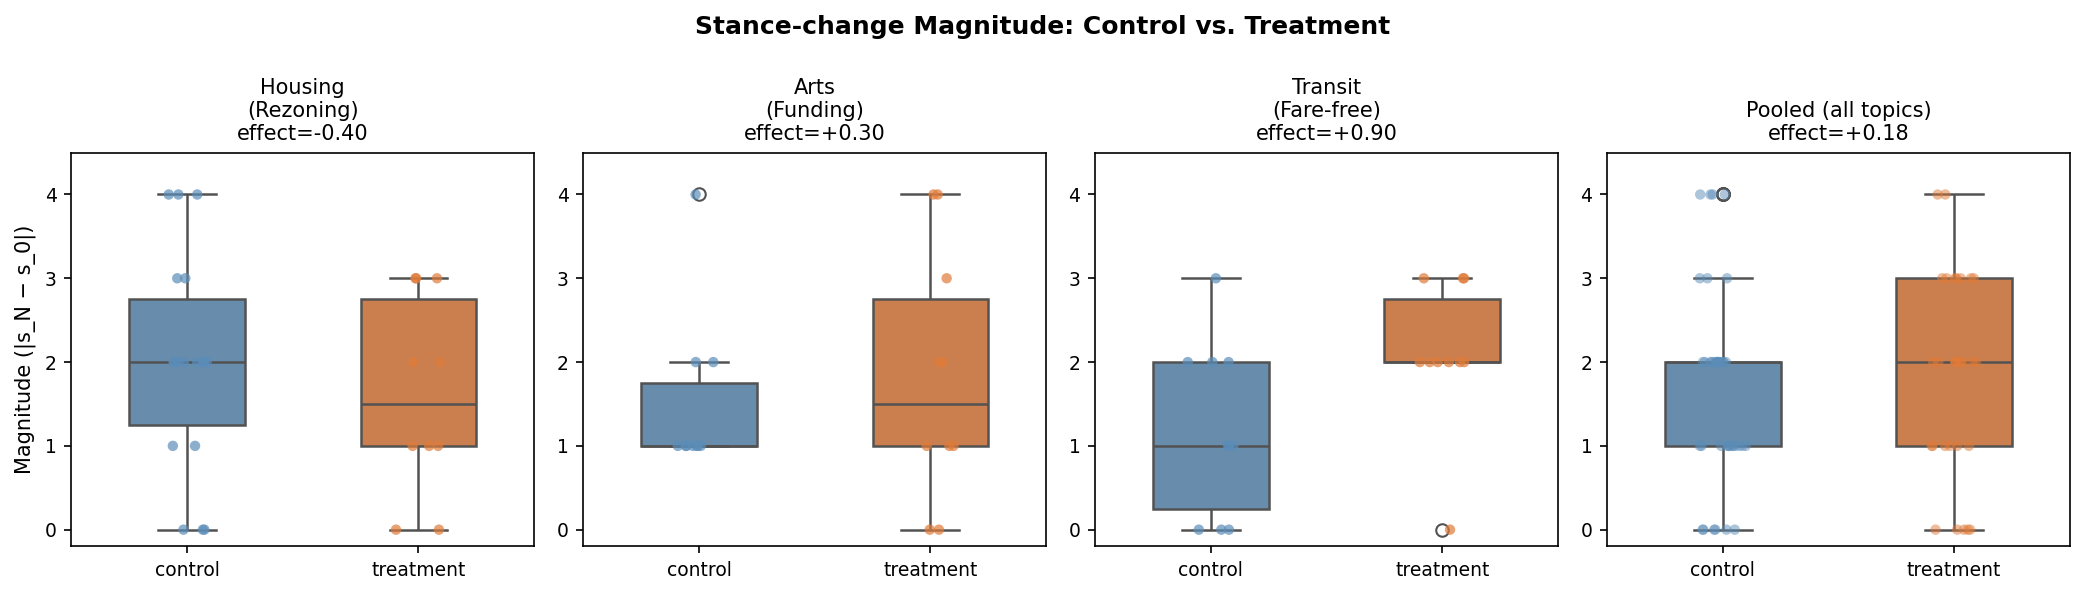
\includegraphics[width=\linewidth]{../results/figures/fig1_magnitude_by_condition.png}
  \caption{Stance-change magnitude distributions by topic and condition.
    Pooled panel (rightmost) shows overlapping distributions with marginally
    higher treatment mean. Magnitude is a secondary metric due to judge scale
    drift on complex propositions.}
  \label{fig:fig1}
\end{figure}

\begin{figure}[h]
  \centering
  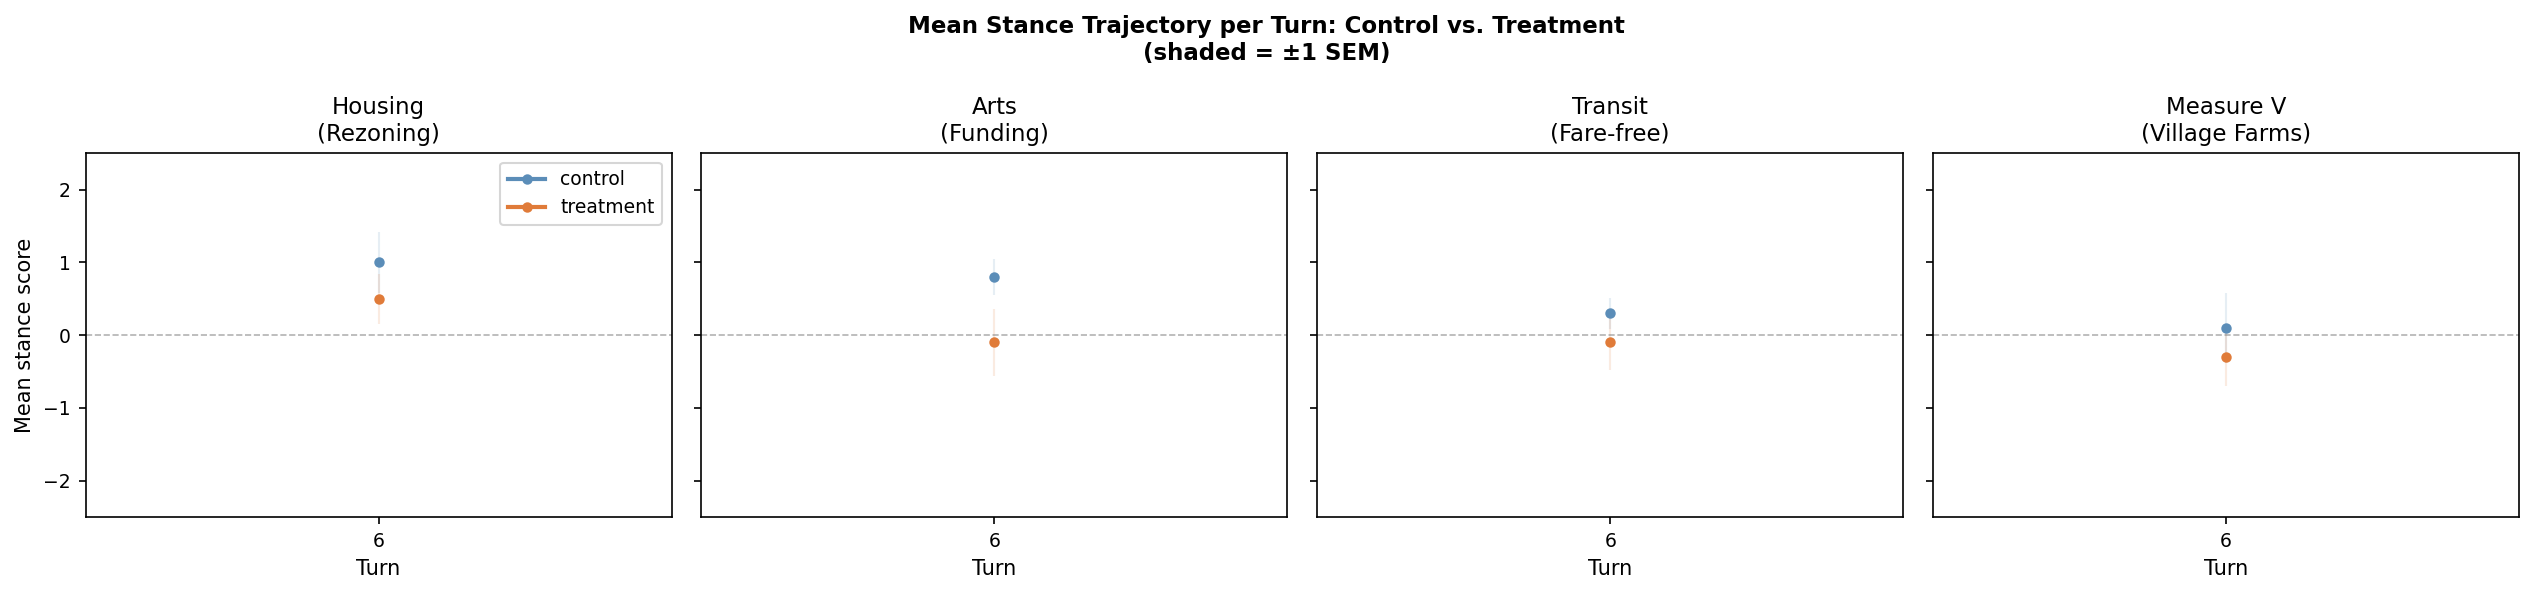
\includegraphics[width=\linewidth]{../results/figures/fig2_trajectories.png}
  \caption{Mean stance by condition and initial suspect stance ($\pm$1 SEM).
    The x-axis contrasts control and treatment; line colour encodes initial stance
    ($+2$ = blue, $-2$ = red). Solid full-colour lines show the mean across turns
    1--6 (post-interrogation); light-colour lines show the turn-0 baseline (before
    the Interrogator has spoken), serving as a reference for how much each group
    moved. Means are computed separately per condition $\times$ initial-stance
    combination. See Figure~\ref{fig:fig3} for directional accuracy.}
  \label{fig:fig2}
\end{figure}

% ─────────────────────────────────────────────────────────────────────────────
\section{Discussion}

\subsection{Why Does Technique Recommendation Help?}
The treatment Interrogator has access to two things the control lacks: (1) a
phase-appropriate technique that shapes \emph{how} to engage (e.g., Scharff
elicitation in the middle phase, which avoids direct contradiction and instead
frames counter-arguments as the Suspect's own conclusions), and (2) retrieved
topic arguments that give the Interrogator factually grounded claims rather than
relying on the base model's parametric knowledge. The combination produces more
coherent, strategically timed responses, which in turn produces more consistent
Suspect movement. We caution that this account is a \emph{hypothesis}: because
the pipeline does not log which technique the selector chose each turn
(Section~\ref{sec:limits}), we cannot verify that the generator actually followed
the selected technique. A manual audit of transcripts (checking technique
adherence on a sample of turns) would be needed to establish the mechanism, and
we leave it to future work.

\subsection{Why Is the Control Below Chance?}
\label{sec:control}
A striking feature of Table~\ref{tab:results} is that pooled control accuracy is
35\%, \emph{below} the 50\% direction-agnostic line, and as low as 10\% on
Transit. The unguided interrogator is therefore, on average, associated with the
suspect moving \emph{away} from its target. We do not have a logged mechanism and
offer three non-exclusive candidate explanations. (i) A \emph{backfire} effect:
unguided, ungrounded argumentation may read as pushy or weak and entrench the
suspect, a well-documented dynamic in human persuasion. (ii)
\emph{Bounded-movement geometry}: suspects start at a stance pole
($d_0 = \pm 2$), so once the Judge scores the opening utterance near that pole
there is little room to move further toward the target and ample room to move
away, biasing the sign of $s_6 - s_0$ against the target under noise. (iii)
\emph{Self-revelation}: against a weak interrogator the suspect may simply
elaborate its initial position, which the Judge reads as movement away. Because
the size of our headline gap depends on control being this low, distinguishing
these explanations, ideally with a neutral-start condition ($d_0 = 0$) that
removes the pole geometry, is important future work.

\subsection{The Arts Exception}
The lack of improvement on the Arts topic is instructive. Arts-funding debates
center on values (``arts enrich communities'', ``public money should fund public
goods''), which are less amenable to the factual-claim structure that the Reid
and Scharff cards target. Our corpus is not, however, devoid of values-applicable
tools: the six structured-debate cards (steelmanning, Socratic questioning) apply
directly to value disagreements, as does the Motivational Interviewing card. The
null result may therefore reflect not a missing capability but a \emph{selection}
failure, with the phase-filtered selector not surfacing those cards (or their
being insufficient on their own). Distinguishing ``wrong tools available'' from
``right tools not selected'' requires the per-turn technique logging we currently
lack (Section~\ref{sec:limits}), and is an interesting question in its own
right.

\subsection{Limitations}
\label{sec:limits}

\textbf{LLM-vs.-LLM evaluation and judge circularity.} All three roles use the
same model family (llama3.1:8b). Estornell and Liu~\cite{estornell2024scaling}
show that shared training distributions introduce correlated biases, but in our
setting the concern is sharper than bias: the same model distribution generates
the suspect's utterances, produces the interrogator's moves, \emph{and} grades
the outcome, so the primary metric is partly circular. A held-out Judge from a
different family (e.g., qwen2.5:7b) is therefore not merely a refinement but a
precondition for fully trusting the absolute numbers. We foreground directional
accuracy precisely because it is the measure least sensitive to the Judge's
absolute calibration, but it does not escape the circularity entirely.

\textbf{Judge scale drift.} On complex propositions (especially Measure V and
Housing), the Judge occasionally scores utterances outside $[-2,2]$ or returns
arrays of incorrect length. We apply clamping and a per-utterance fallback,
but the underlying instability inflates variance in the magnitude metric.
Directional accuracy is substantially more robust.

\textbf{Small \textit{N} and independence.} The pooled comparison (40 legs per condition)
is statistically significant ($z=3.6$, $p<0.001$), but per-topic comparisons
($n=10$) are not powered for significance testing, so individual topic rankings
are indicative only. The five quads within a topic use distinct seeds (42--46),
yet the same five seeds recur across topics and the two conditions are matched
within a quad, so treating the 80 legs as fully independent is an approximation;
a larger, fully-crossed run is needed to tighten the estimates.

\textbf{Technique vs.\ argument confound.} The treatment condition adds two
things the control lacks: technique guidance (Channel~1) and retrieved topic
arguments (Channel~2). Our design therefore measures their combined effect and
cannot isolate the contribution of technique selection on its own. The natural
ablation, an arguments-only condition that supplies Channel~2 without Channel~1,
would separate the two; we leave it for future work.

\textbf{Technique logging gap.} The current pipeline does not write the
selected technique back to the transcript, preventing post-hoc analysis of
which techniques were most effective or most frequently selected. This limits
our ability to close the recommendation loop and identify underperforming
technique cards.

\textbf{Single-topic real dataset.} Measure V is one real topic. A fuller
evaluation would use a set of real ballot measures (or social media arguments)
across a wider domain range.

\textbf{Benign topics vs.\ extremist framing.} Our motivation invokes online
extremism and entrenched belief, but we evaluate on low-affect civic ballot
measures chosen for neutrality and reproducibility. Genuinely extremist or
identity-protective stances may resist persuasion through mechanisms (motivated
reasoning, identity threat) that are weak or absent here. Our results are
therefore best read as evidence about controlled stance change: a proxy for, not
a direct test of, moderating entrenched or extremist views.

\subsection{Ethical Considerations}
This system is designed as a research tool for studying LLM persuasion
dynamics, not for deployment against real humans without consent. Techniques
drawn from the Reid framework in particular have been criticized for producing
false confessions in real interrogation contexts~\cite{leo2008police}; in our
setting they are applied to LLM-simulated suspects in a controlled evaluation.
Deployment in any real moderation context would require independent safety
review, consent mechanisms, and domain-specific calibration. More broadly, the
interrogation framing we borrow from, while technically precise for our
technique corpus, can obscure the underlying intent: to create the conditions
for genuine reconsideration. A responsible deployment would treat individuals
with entrenched views not as targets to be argued into submission, but as people
who may have unmet social, psychological, or informational needs. A well-designed
system should be capable of shifting from structured dialogue toward supportive,
motivational exchange when such needs emerge.

% ─────────────────────────────────────────────────────────────────────────────
\section{Conclusion}

We have shown that a RAG-powered technique recommender improves LLM
interrogator performance on a stance-change task across four ballot-measure
topics, including one real-world dataset (Davis Measure V). The treatment
condition achieves 75\% directional accuracy versus 35\% for the unguided
control, a 40-percentage-point improvement ($p<0.001$, pooled); the largest
single-topic gap is Transit (10\% $\to$ 90\%), though per-topic samples are
small. Technique recommendation also improves stance consistency, suggesting
coherent directional influence rather than noise-driven oscillation. The real-data condition (Measure V)
replicates the improvement despite substantially richer and more complex
argument structure, supporting the generalizability of the approach.

The primary limitation is the LLM-vs.-LLM evaluation setting, which introduces
shared-bias confounds. Future work should add an arguments-only condition to
isolate the technique channel from the argument channel, evaluate with a held-out
Judge model, instrument the system to log selected techniques per turn, and
expand the real-data condition to a broader set of genuine public-debate topics.

A broader extension would connect this system to network-scale intervention.
Research on online ideological communities shows that influence spreads
non-uniformly: a small number of high-centrality actors account for a
disproportionate share of content propagation~\cite{ribeiro2018sheep}, and
dynamic graph-learning tools~\cite{yu2023dygformer, sun2023explicit} can model
how such influence evolves over time. A natural extension would pair network
analysis with our dialogue recommender, first identifying likely-responsive
high-centrality individuals, then initiating technique-guided conversations with
them. We must, however, flag an unresolved tension with the consent principle in
our Ethical Considerations: deploying technique-guided persuasion against
non-consenting, network-selected targets would be manipulation at scale, which we
do not endorse. We frame this direction as legitimate only under transparency and
opt-in conditions (for example, users who have explicitly requested a debate
partner, or platform tools that disclose the system's nature and purpose).
Resolving this tension is a prerequisite to any real deployment, not an
afterthought.

% ─────────────────────────────────────────────────────────────────────────────
\section{Contribution Statement}
Each member wrote their own contribution statement.

\textbf{Marcin Wróblewski}: Initiated the project and its core research idea
(using real-world interrogation techniques to moderate extremist stances).
Proposed the overall three-role multi-agent architecture (Suspect, Interrogator,
Judge), the quad-based experimental design, and the real-data generalization test
(the Davis Measure~V condition). Led the team and organized the collaborative
working meetings, and maintained the project's GitHub infrastructure. Finalized
the slides for the final presentation. Contributed to revising the paper.

\textbf{Haoyu Yan}: Implemented the entire codebase realizing the team's designs:
the LLM client (Ollama HTTP wrapper); the three roles, including the
Interrogator's control branch and two-stage RAG treatment pipeline; the
two-channel RAG recommender (18 technique cards, topic cards, ChromaDB index, and
phase-aware retrievers); the quad experiment runner; the metrics; the analysis
scripts and figures; and the Measure~V data integration. Authored the full paper
draft in ACM format (iterative revisions, citation verification, significance
analysis, and limitations) and drafted the presentation slides. Contributed to
revising the paper.

\textbf{Bill Steeven Koumba Moussadji Lu}: Proposed the evaluation methodology: the magnitude,
direction, and consistency metrics and the worked-example Judge scoring scheme.
Led the interpretation of the experimental results during the working meetings.
Gave detailed editorial review of the paper drafts, with stylistic and structural
suggestions that were incorporated into the final version, and reviewed and
refined the presentation slides. Contributed to revising the paper.

{\sloppy
\textbf{Sanjay Manivasagam}: Built the project's cross-OS portability layer:
cross-platform Ollama discovery (scripts/ollama\_runtime.py), the UTF-8 console
fix for Windows, the one-command setup.py bootstrap, the CI matrix
(Ubuntu/macOS/Windows $\times$ Python 3.11--3.12), and the portability audit
(docs/PORTABILITY.md), enabling reproducible runs on all three operating systems.
Authored the project README and contributed early architectural sourcing for the
two-agent dialogue design. Conducted a methodological peer review of the paper
(judge-independence, the techniques-vs-arguments confound, significance testing,
and ablation gaps). Owns the Experimental Design and Evaluation Metrics
presentation sections.\par}

% ─────────────────────────────────────────────────────────────────────────────
\section{Meeting Participation}
Much of the project's progress was made collaboratively during the team's working
meetings. We note attendance below as one objective reference point.

\begin{table}[h]
\centering
\begin{tabular}{lc}
\toprule
Member & Meetings attended \\
\midrule
Marcin Wróblewski & 16 \\
Haoyu Yan & 12 \\
Bill Steeven Koumba Moussadji Lu & 9 \\
Sanjay Manivasagam & 5 \\
\bottomrule
\end{tabular}
\end{table}

% ─────────────────────────────────────────────────────────────────────────────
\bibliographystyle{ACM-Reference-Format}
\begin{thebibliography}{10}

\bibitem{costello2024durably}
Thomas H. Costello, Gordon Pennycook, and David G. Rand. 2024.
\newblock Durably reducing conspiracy beliefs through dialogues with AI.
\newblock \emph{Science} 385, 6714 (2024).

\bibitem{estornell2024scaling}
Andrew Estornell and Yang Liu. 2024.
\newblock Multi-LLM Debate: Framework, Principals, and Interventions.
\newblock In \emph{Advances in Neural Information Processing Systems 37 (NeurIPS 2024)}.

\bibitem{gorwa2020algorithmic}
Robert Gorwa, Reuben Binns, and Christian Katzenbach. 2020.
\newblock Algorithmic content moderation: Technical and political challenges in
  the automation of platform governance.
\newblock \emph{Big Data \& Society} 7, 1 (2020).

\bibitem{hong2024curiosity}
Zhang-Wei Hong, Idan Shenfeld, Tsun-Hsuan Wang, Yung-Sung Chuang, Aldo Pareja,
  James Glass, Akash Srivastava, and Pulkit Agrawal. 2024.
\newblock Curiosity-driven Red-teaming for Large Language Models.
\newblock In \emph{International Conference on Learning Representations (ICLR 2024)}.

\bibitem{izacard2022few}
Gautier Izacard, Patrick Lewis, Maria Lomeli, Lucas Hosseini, Fabio Petroni,
  Timo Schick, Jane Dwivedi-Yu, Armand Joulin, Sebastian Riedel, and Edouard
  Grave. 2023.
\newblock Atlas: Few-shot Learning with Retrieval Augmented Language Models.
\newblock \emph{Journal of Machine Learning Research} 24, 251 (2023), 1--43.

\bibitem{kumar2023language}
Deepak Kumar, Yousef AbuHashem, and Zakir Durumeric. 2023.
\newblock Watch Your Language: Investigating Content Moderation with Large
  Language Models.
\newblock arXiv:2309.14517 (2023).

\bibitem{leo2008police}
Richard A. Leo. 2008.
\newblock \emph{Police Interrogation and American Justice}.
\newblock Harvard University Press.

\bibitem{oleszkiewicz2014scharff}
Sonja Oleszkiewicz, P\"{a}r Anders Granhag, and Steven M. Kleinman. 2014.
\newblock On Eliciting Intelligence from Human Sources: Contextualizing the
  Scharff-Technique.
\newblock \emph{Applied Cognitive Psychology} 28, 6 (2014), 898--907.

\bibitem{ribeiro2018sheep}
Manoel Horta Ribeiro, Pedro H. Calais, Yuri A. Santos, Virg\'ilio A. F. Almeida,
  and Wagner Meira Jr. 2018.
\newblock ``Like Sheep Among Wolves'': Characterizing Hateful Users on Twitter.
\newblock arXiv:1801.00317 (2018).

\bibitem{sun2023explicit}
Xigang Sun, Jingya Zhou, Ling Liu, and Wenqi Wei. 2023.
\newblock Explicit Time Embedding Based Cascade Attention Network for Information
  Popularity Prediction.
\newblock \emph{Information Processing \& Management} 60, 3 (2023), 103278.

\bibitem{yu2023dygformer}
Le Yu, Leilei Sun, Bowen Du, and Weifeng Lv. 2023.
\newblock Towards Better Dynamic Graph Learning: New Architecture and Unified
  Library.
\newblock In \emph{Advances in Neural Information Processing Systems (NeurIPS 2023)}.

\end{thebibliography}

\end{document}
